% \documentclass[12pt, a4paper]{article}

% % --- Essential Packages ---
% \usepackage{xeCJK} % Support for Chinese, Japanese, and Korean
% \usepackage{geometry} % For page margins
% \usepackage{hyperref} % For clickable links and PDF bookmarks

% % --- Font Settings ---
% % Replace "PingFang TC" or "Microsoft JhengHei" with a font installed on your system
% \setCJKmainfont{Noto Sans CJK TC}
% %\setCJKmainfont{PingFang TC} % Common for Mac users

% \geometry{left=2.5cm, right=2.5cm, top=2.5cm, bottom=2.5cm}

% % --- Metadata ---
% \title{Probability HW3}
% \author{B13902022 賴昱錡}
% \date{\today}

% \begin{document}

% \maketitle

% \section*{2.5-5}
% % Your solution here
% Recall that:
% \begin{itemize}
%     \item $M(0)=E[e^{0X}]=E[1]=1$
%     \item $M'(0)=\mu=E[X]$
%     \item $M''(0)=E[X^2]$
% \end{itemize}
% Thus, we obtain:
% \begin{align*}
    
% \end{align*}

% \section*{2.5-6}
% % Your solution here

% \section*{2.6-11}
% % Your solution here

% \section*{3.1-8}
% % Your solution here

% \section*{3.2-4}
% % Your solution here

% \end{document}
\documentclass[12pt]{article}
\usepackage{graphicx}
\usepackage[margin=2cm, a4paper]{geometry}
\usepackage{setspace}
\usepackage{pdfpages}
\usepackage{float}
\usepackage{amsmath}
\usepackage{fancyvrb}
\usepackage{amssymb}
\usepackage{minted}
\usepackage{enumitem}
\usepackage[colorlinks,linkcolor=blue]{hyperref}


\renewcommand{\contentsname}{Contents}
\renewcommand{\figurename}{Figure}
\renewcommand{\tablename}{Table}
\hypersetup{
    colorlinks=true,
    linkcolor=black,
    filecolor=magenta,      
    urlcolor=blue,
}
\newcommand{\mytitle}{Probability - Homework 3}
\newcommand{\myauthor}{B13902022 Yu-Chi,Lai}

\usepackage{fancyhdr}
\pagestyle{fancy}
\fancyhead{}
\fancyhead[L]{\mytitle}
\fancyhead[R]{\myauthor}

\usepackage[english]{babel}
\usepackage{amsthm}

\newtheorem{theorem}{Theorem}[section]
\newtheorem{corollary}[theorem]{Corollary}
\newtheorem{lemma}[theorem]{Lemma}

\theoremstyle{definition}
\newtheorem{definition}{Definition}[section]
\theoremstyle{remark}
\newtheorem*{remark}{Remark}

\title{\mytitle}
\author{\textbf{\myauthor}}
\date{}

\begin{document}

\maketitle

\section*{2.5-5}
% Your solution here
Recall that:
\begin{itemize}
    \item $M(0)=E[e^{0X}]=E[1]=1$
    \item $M'(0)=\mu=E[X]$
    \item $M''(0)=E[X^2]$
\end{itemize}
Thus, we obtain:
\begin{align*}
    R'(0)=\frac{M'(0)}{M(0)}=\frac{\mu}{1}=\mu \\
    R''(0)=\frac{M(0)M''(0)-[M'(0)]^2}{[M(0)]^2}=\frac{1\cdot E[X^2]-(E[X])^2}{1}=E[X^2]-(E[X])^2=\sigma^2
\end{align*}
completes the proof

\section*{2.5-6}
% Your solution here
\subsection*{(a)}
Suppose the probability of success be $p$, $X$ be the r.v. standing for the number of success.
$$M(t)=P(X=0)\cdot e^{0t}+P(X=1)\cdot e^{1t}=(1-p)+p\cdot e^t$$

Then we have:
\begin{align*}
    R(t)=\ln{(1-p+pe^t)} \\
    R'(t)=\frac{pe^t}{1-p+pe^t} \\
    R''(t)=\frac{(1-p+pe^t)pe^t-(pe^t)^2}{(1-p+pe^t)^2}
\end{align*}

By the results in 2.5-5, $\mu=R'(0)=p$, $\sigma^2=R''(0)=p(1-p)$
\subsection*{(b)}
Suppose the probability of success be $p$, $X$ be the r.v. standing for the number of success, and $n$ be the count of the trials.
\begin{align*}
    M(t)&=\sum^n_{k=0}\binom{n}{k}p^k(1-p)^{n-k}e^{kt} \\
    &=\sum^n_{k=0}\binom{n}{k}(pe^t)^k(1-p)^{n-k} \\
    &=(1-p+pe^t)^n
\end{align*}
The last equation comes from binomial theorem. And the first and second derivatives are:
\begin{align*}
    M'(t)=n(1-p+pe^t)^{n-1}pe^t \\
    M''(t)=n(n-1)(1-p+pe^t)^{n-2}(pe^t)^2+n(1-p+pe^t)^{n-1}pe^t
\end{align*}
Hence, since $R(t)=\ln M(t)=n\ln(1-p+pe^t)$,
\begin{align*}
    R'(t)&=\frac{npe^t}{1-p+pe^t} \\
    R''(t)&=\frac{npe^t(1-p)}{(1-p+pe^t)^2}
\end{align*}
By the results in 2.5-5, $\mu=R'(0)=np$ and $\sigma^2=R''(0)=np(1-p)$.
\subsection*{(c)}
Suppose the probability of success be $p$, $X$ be the r.v. standing for the number of trials to observe one success.

\begin{align*}
    M(t)&=\sum_{k=1}^{\infty}e^{kt}(1-p)^{k-1}p \\
    &=pe^t\sum_{k=1}^{\infty}(e^t(1-p))^{k-1} \\
    &=\frac{pe^t}{1-e^t(1-p)}
\end{align*}

With the bound for $t$:
$$e^t<\frac{1}{1-p}\Rightarrow t<-\ln{(1-p)}$$

Hence, we have:
\begin{align*}
    R(t)&=\ln{(\frac{pe^t}{1-e^t(1-p)})} \\
    R'(t)&=\frac{1-e^t(1-p)}{pe^t}\cdot \frac{pe^t(1-e^t(1-p))+p(1-p)e^{2t}}{[1-e^t(1-p)]^2} \\
    &=\frac{(1-e^t(1-p))+(1-p)e^t}{1-e^t(1-p)} \\
    &=1+\frac{(1-p)e^t}{1-e^t(1-p)} \\
    R''(t)&=\frac{(1-p)e^t[1-e^t(1-p)]+[(1-p)e^t]^2}{[(1-e^t(1-p))]^2}
\end{align*}
By some calculation, we found $\mu=R'(0)=\frac{1}{p}$ and $\sigma^2=\frac{(1-p)p+(1-p)^2}{p^2}=\frac{1-p}{p^2}$
\subsection*{(d)}
\noindent\makebox[\linewidth]{\rule{\linewidth}{0.4pt}}
\begin{theorem}
The expected values of two random variables is multiplicative if \textbf{they are indenpendent}, i.e., $E[XY]=E[X][Y]$
\end{theorem}
\begin{proof}
If $X$ and $Y$ are independent (and $\mathcal{X}$ and $\mathcal{Y}$ are the sample spaces for $X$ and $Y$ respectively.), it holds that

\begin{equation}
p(x, y) = p(x)p(y) \quad \text{for all} \quad x \in \mathcal{X}, y \in \mathcal{Y} .
\end{equation}

Applying this to the expected value for discrete random variables, we have

\begin{align*}
\text{E}(XY) &= \sum_{x \in \mathcal{X}} \sum_{y \in \mathcal{Y}} (x \cdot y) \cdot f_{X,Y}(x, y) \\ 
&= \sum_{x \in \mathcal{X}} \sum_{y \in \mathcal{Y}} (x \cdot y) \cdot (f_X(x) \cdot f_Y(y)) \\ 
&= \sum_{x \in \mathcal{X}} x \cdot f_X(x) \sum_{y \in \mathcal{Y}} y \cdot f_Y(y) \\ 
&= \sum_{x \in \mathcal{X}} x \cdot f_X(x) \cdot \text{E}(Y) \\ 
&= \text{E}(X)\text{E}(Y) . 
\end{align*}

And applying it to the expected value for continuous random variables, we have

\begin{align*} 
\text{E}(XY) &= \int_{\mathcal{X}} \int_{\mathcal{Y}} (x \cdot y) \cdot f_{X,Y}(x, y) \,dy \,dx \\ 
&= \int_{\mathcal{X}} \int_{\mathcal{Y}} (x \cdot y) \cdot (f_X(x) \cdot f_Y(y)) \,dy \,dx \\ 
&= \int_{\mathcal{X}} x \cdot f_X(x) \int_{\mathcal{Y}} y \cdot f_Y(y) \,dy \,dx \\ 
&= \int_{\mathcal{X}} x \cdot f_X(x) \cdot \text{E}(Y) \,dx \\ 
&= \text{E}(X)\text{E}(Y) . 
\end{align*}
\end{proof}

\noindent\makebox[\linewidth]{\rule{\linewidth}{0.4pt}}

Let $Y$ be the r.v. for the number of trials to achiving exactly $r$ successes.

We can express $Y$ as the sum of $r$ independent, identically distributed geometric random variables, $p$ is the probability of getting success in a single test:
$$Y=X_1+X_2+\dots+X_r$$
In this equation, $X_1$ is the number of trials to get the first success, $X_2$ is the number of additional trials to get the second success, and so on up to the $r$-th success.

As derived previously, the m.g.f for a single geometric r.v. is:
$$M_X(t)=\frac{pe^t}{1-e^t(1-p)}$$

By Theorem 0.1, we can obtain the m.g.f for $Y$ using following steps:
\begin{align*}
M_Y(t)&=E[e^{Yt}] \\
&=E[e^{(X_1+X_2+\dots+X_r)}] \\
&=E[e^{X_1t}\cdot e^{X_2t}\cdot\dots\cdot e^{X_rt}] \\
&=E[e^{X_1t}]E[e^{X_2t}]\dots E[e^{X_rt}] \\
&=(\frac{pe^t}{1-e^t(1-p)})^r
\end{align*}
Then let's derive $R(t)$, and its first and second derivatives:
\begin{align*}
    R(t)&=\ln{(M_Y(t))} \\
    &=r(\ln{(p)}+t-\ln{(1-e^t(1-p))}) \\
    R'(t)&=r(1+\frac{(1-p)e^t}{1-e^t(1-p)}) \\
    R''(t)&=r\frac{(1-p)e^t[1-e^t(1-p)]+[e^t(1-p)]^2}{[1-e^t(1-p)]^2} \\
    &=r\frac{(1-p)e^t}{[1-e^t(1-p)]^2}
\end{align*}
By some easy calculation, we know $\mu=R'(0)=\frac{r}{p}$ and $\sigma^2=R''(0)=\frac{r(1-p)}{p^2}$
\section*{2.6-11}
% Your solution here
Let $Y$ be the number of passengers who do not show up. Since the probability of a passenger not showing up is $0.05$ and we are assuming independence, $Y$ follows a Binomial distribution: $Y \sim \text{Binomial}(n=100, p=0.05)$.

\subsection*{(b)}
For the airline to fit everyone on the plane, the number of passengers who actually arrive must be 95 or fewer. That means out of the 100 tickets sold, at least 5 people must fail to show up. 

So, we want to find the probability that $Y \ge 5$:
$$P(Y \ge 5) = 1 - P(Y \le 4)$$

To find $P(Y \le 4)$, we sum the binomial probabilities from $y=0$ to $y=4$ using the formula $P(Y=y) = \binom{n}{y} p^y (1-p)^{n-y}$:
\begin{itemize}
    \item $P(Y=0) = \binom{100}{0}(0.05)^0(0.95)^{100} \approx 0.0059$
    \item $P(Y=1) = \binom{100}{1}(0.05)^1(0.95)^{99} \approx 0.0312$
    \item $P(Y=2) = \binom{100}{2}(0.05)^2(0.95)^{98} \approx 0.0812$
    \item $P(Y=3) = \binom{100}{3}(0.05)^3(0.95)^{97} \approx 0.1396$
    \item $P(Y=4) = \binom{100}{4}(0.05)^4(0.95)^{96} \approx 0.1781$
\end{itemize}

Summing those probabilities gives us $P(Y \le 4) \approx 0.4360$. 
Now, substitute that back into our original equation:
$$P(Y \ge 5) = 1 - 0.4360 = 0.5640$$

\textbf{Answer:} There is approximately a 56.4\% chance the airline can accommodate everyone.

\vspace{1em}

\subsection*{(b)}

If the airline has to turn a passenger away, they must refund the \$300 ticket price plus pay a \$400 penalty. That means the cost per bumped passenger is \$700.

Passengers get bumped if fewer than 5 people fail to show up (i.e., when $Y < 5$). Let's find the expected number of bumped passengers:
\begin{itemize}
    \item If $Y=4$ (96 show up), 1 passenger is bumped.
    \item If $Y=3$ (97 show up), 2 passengers are bumped.
    \item If $Y=2$ (98 show up), 3 passengers are bumped.
    \item If $Y=1$ (99 show up), 4 passengers are bumped.
    \item If $Y=0$ (100 show up), 5 passengers are bumped.
\end{itemize}

We calculate the expected number of bumped passengers, $E[\text{Bumped}]$, by multiplying each outcome by its probability:
$$E[\text{Bumped}] = \sum_{y=0}^{4} (5-y) \cdot P(Y=y)$$
$$E[\text{Bumped}] = 5(0.0059) + 4(0.0312) + 3(0.0812) + 2(0.1396) + 1(0.1781) \approx 0.8551$$

Now, multiply the expected number of bumped passengers by the \$700 cost to find the total expected payout:
$$\text{Expected Payout} = 700 \times 0.8551 = 598.57$$

\textbf{Answer:} The airline's expected payout is approximately \$598.57.
\section*{3.1-8}
% Your solution here
\subsection*{Part (a): $f(x) = x^3/4,\quad 0 < x < c$}

\noindent\textbf{(i) Find $c$:}
\[
\int_0^c \frac{x^3}{4}\,dx = \frac{c^4}{16} = 1 \implies c^4 = 16 \implies c = 2
\]

\noindent\textbf{(ii) CDF:}
\[
F(x) = \int_0^x \frac{t^3}{4}\,dt = \frac{x^4}{16}, \quad 0 < x < 2
\]

\noindent\textbf{(iv) Mean and Variance:}
\[
\mu = \int_0^2 x \cdot \frac{x^3}{4}\,dx = \frac{1}{4}\cdot\frac{x^5}{5}\Bigg|_0^2 = \frac{32}{20} = \frac{8}{5}
\]
\[
E[X^2] = \int_0^2 x^2 \cdot \frac{x^3}{4}\,dx = \frac{1}{4}\cdot\frac{x^6}{6}\Bigg|_0^2 = \frac{64}{24} = \frac{8}{3}
\]
\[
\sigma^2 = E[X^2] - \mu^2 = \frac{8}{3} - \frac{64}{25} = \frac{8}{75}
\]

\subsection*{Part (b): $f(x) = \frac{3}{16}x^2,\quad -c < x < c$}

\noindent\textbf{(i) Find $c$:}
\[
\int_{-c}^{c} \frac{3}{16}x^2\,dx = \frac{3}{16}\cdot\frac{2c^3}{3} = \frac{c^3}{8} = 1 \implies c = 2
\]

\noindent\textbf{(ii) CDF:}
\[
F(x) = \int_{-2}^{x} \frac{3}{16}t^2\,dt = \frac{x^3 + 8}{16}, \quad -2 < x < 2
\]

\noindent\textbf{(iv) Mean and Variance:}\\
Since $f(x)$ is symmetric about 0:
\[
\mu = 0
\]
\[
\sigma^2 = E[X^2] = \int_{-2}^{2} x^2 \cdot \frac{3}{16}x^2\,dx = \frac{3}{8}\cdot\frac{32}{5} = \frac{12}{5}
\]

\subsection*{Part (c): $f(x) = c/\sqrt{x},\quad 0 < x < 1$}

\noindent\textbf{(i) Find $c$:}
\[
\int_0^1 \frac{c}{\sqrt{x}}\,dx = 2c = 1 \implies c = \frac{1}{2}
\]
The pdf is \textbf{unbounded} since $f(x) \to \infty$ as $x \to 0^+$.

\noindent\textbf{(ii) CDF:}
\[
F(x) = \int_0^x \frac{1}{2\sqrt{t}}\,dt = \sqrt{x}, \quad 0 < x < 1
\]

\noindent\textbf{(iv) Mean and Variance:}
\[
\mu = \int_0^1 x \cdot \frac{1}{2\sqrt{x}}\,dx = \frac{1}{2}\int_0^1 x^{1/2}\,dx = \frac{1}{3}
\]
\[
E[X^2] = \frac{1}{2}\int_0^1 x^{3/2}\,dx = \frac{1}{5}
\]
\[
\sigma^2 = \frac{1}{5} - \frac{1}{9} = \frac{4}{45}
\]

\noindent\makebox[\linewidth]{\rule{\linewidth}{0.4pt}}

\noindent\textbf{(iii)}
\begin{figure}[H]
    \centering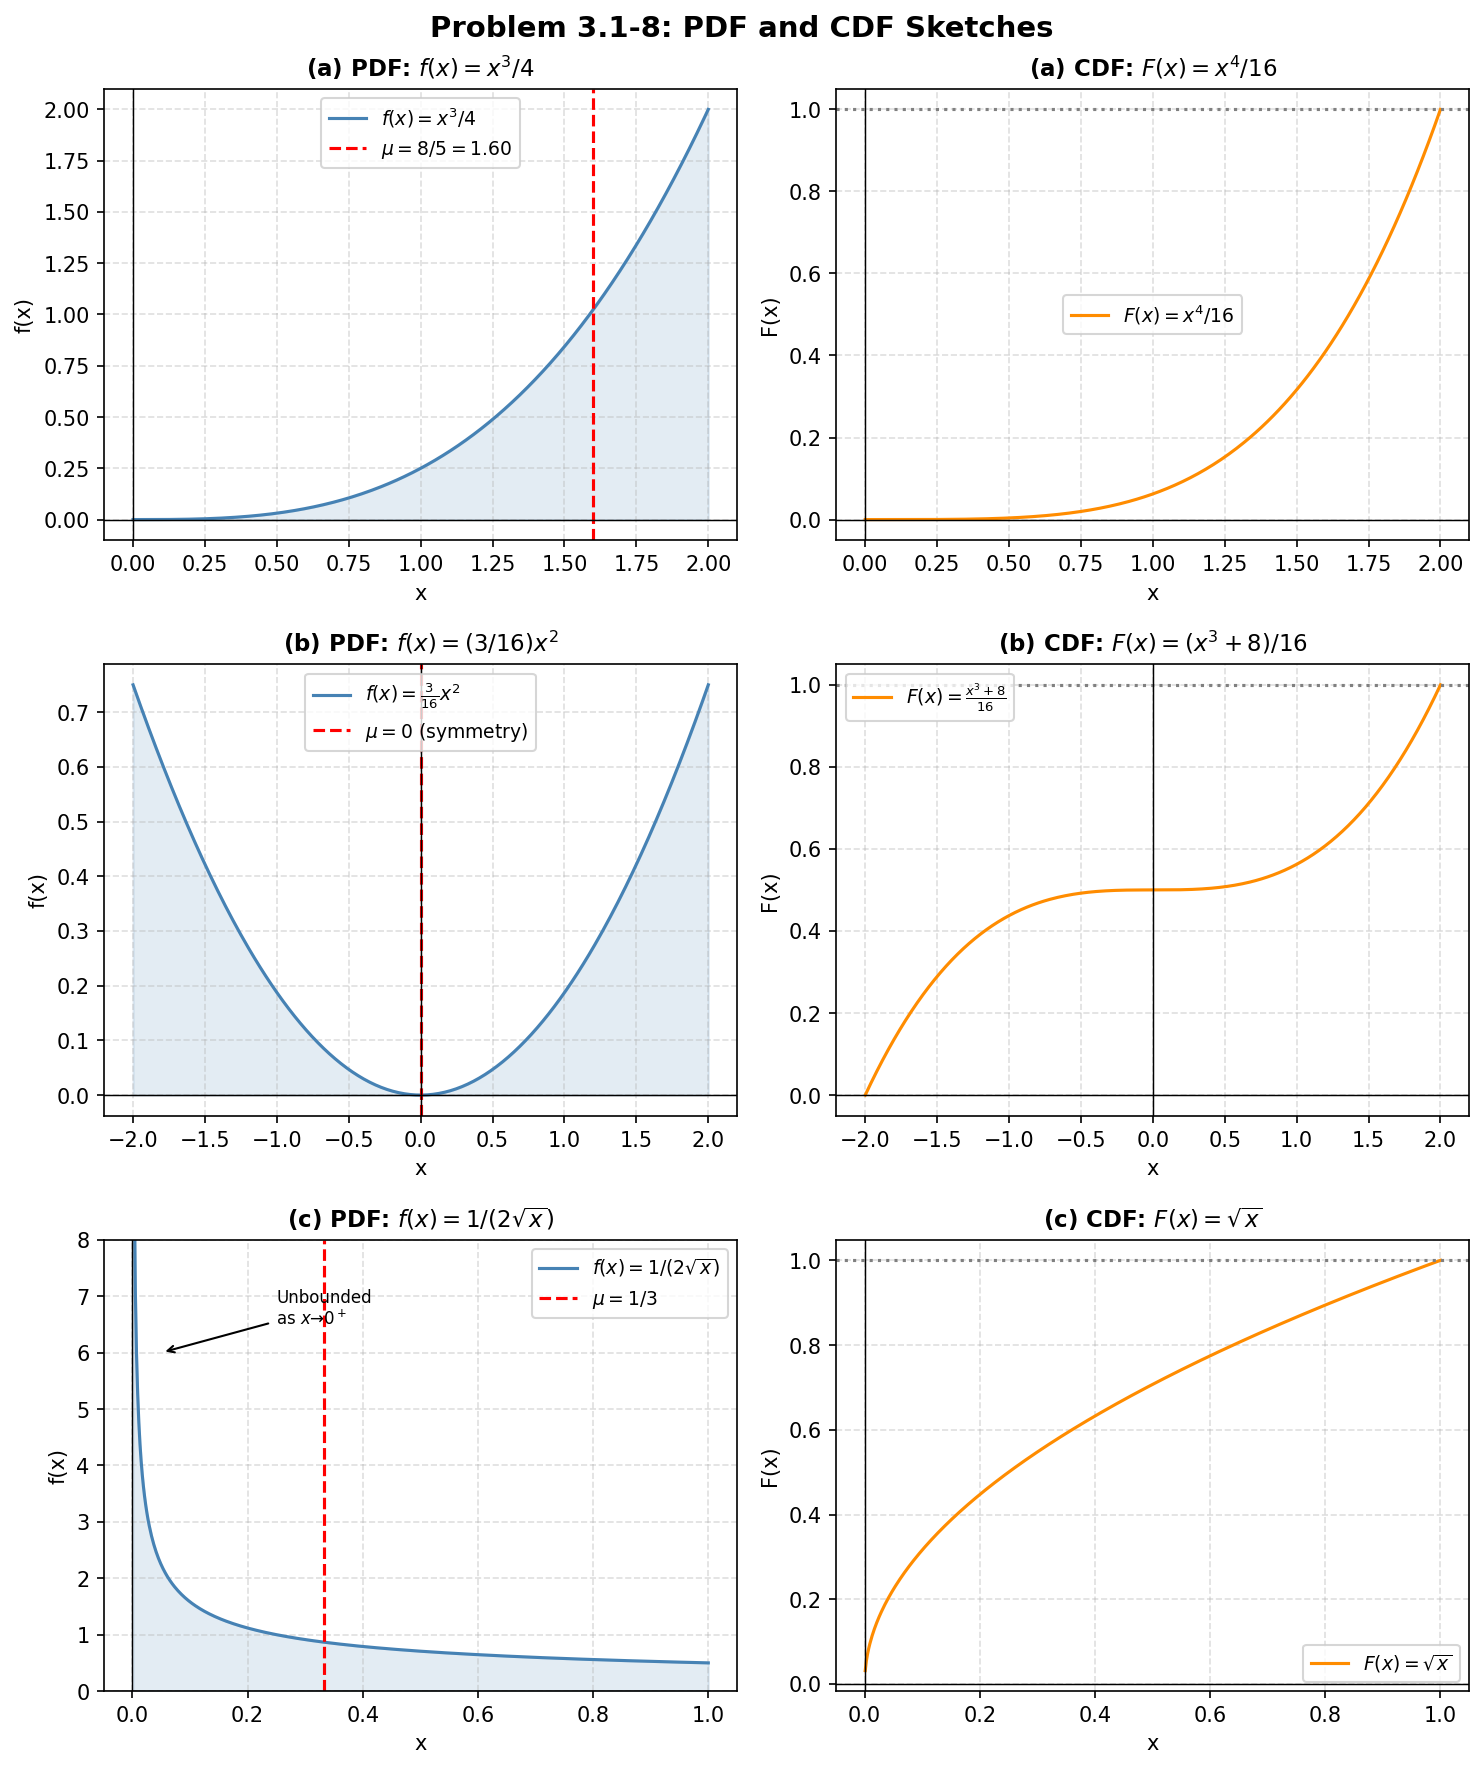
\includegraphics[width=\linewidth]{hw3_problem4.png}
    \caption{All the graphs in problem 3.1-8}
\end{figure}

\section*{3.2-4}
% Your solution here
Let $X$ be a continuous-type random variable with cdf $F(x)$, where $F(x)=0$ for $x\le0$ and $0<F(x)<1$ for $0<x$.

We are given the conditional probability:
$$P(X > x+y \mid X > x) = P(X > y)$$

Using the definition of conditional probability, we have:
$$\frac{P(X > x+y \cap X > x)}{P(X > x)} = P(X > y)$$

Since $x > 0$ and $y > 0$, the event $(X > x+y)$ is a strict subset of $(X > x)$. Therefore, the intersection $(X > x+y \cap X > x)$ simplifies to $(X > x+y)$. Substituting this back gives:
$$\frac{P(X > x+y)}{P(X > x)} = P(X > y)$$
$$P(X > x+y) = P(X > x)P(X > y)$$

Following the hint, let $g(x) = 1 - F(x) = P(X > x)$. Substituting $g$ into the equation yields:
$$g(x+y) = g(x)g(y)$$

This is Cauchy's functional equation. Its only continuous, non-trivial solution is of the form $g(x) = e^{kx}$. 

Because $0 < F(x) < 1$ for $x > 0$, it follows that $0 < g(x) < 1$ for $x > 0$. For $e^{kx}$ to be strictly between 0 and 1 for positive $x$, the constant $k$ must be negative. Let $k = -\lambda$ for some constant $\lambda > 0$. Thus:
$$g(x) = e^{-\lambda x}$$

Finally, substitute $g(x)$ back into the expression for $F(x)$:
$$F(x) = 1 - g(x) = 1 - e^{-\lambda x}, \quad 0 < x$$

This completes the proof.

\end{document}
% how to display codes?
% \begin{minted}[frame=lines,framesep=2mm,baselinestretch=1.2,linenos,breaklines]{python}
% \end{minted}

% how to display images?
% \begin{figure}[H]
%     \centering
%     \includegraphics[width=0.5\linewidth]{}
%     \caption{Caption}
% \end{figure}
% test